
\section{\label{sec:Tutorial-Greensfns-2d}Tutorial Generating and Using Green's
Functions in Two Dimensions}

PyLith features discussed in this tutorial:
\begin{itemize}
\item Green's functions
\item HDF5 output
\item HDF5 point output
\item Reading HDF5 output using h5py
\item Simple inversion procedure
\item Plotting results using matplotlib
\item Cubit mesh generation

\begin{itemize}
\item Variable mesh resolution
\item APREPRO programming language
\end{itemize}
\item Static solution
\item Linear triangular cells
\item Kinematic fault interface conditions
\item Plane strain linearly elastic material
\item SimpleDB spatial database
\item ZeroDispDB spatial database
\item UniformDB spatial database
\end{itemize}
All of the files necessary to run the examples are contained under
the directory \texttt{examples/2d/greensfns.}


\subsection{Overview}

This tutorial examines the steps necessary to generate Green's functions
using PyLith and how they may be used in a linear inversion. For simplicity
we discuss strike-slip and reverse faulting examples in the context
of 2D simulations. In each example, we first compute surface displacement
at a set of points, and these computed displacements provide the ``data''
for our inversion. Second, we compute a set of Green's functions using
the same fault geometries, and output the results at the same set
of points. Third, we perform a simple linear inversion. An important
aspect for both the forward problem and the Green's function problem
is that the computed solution is output at a set of user-specified
points (not necessarily coincident with mesh vertices), rather than
over a mesh or sub-mesh as for other types of output. To do this,
PyLith internally performs the necessary interpolation. There is a
README file in the top-level directory that explains how to perform
each step in the two problems.


\subsection{Mesh Description}

We use linear triangular cells for the meshes in each of the two problems.
We construct the mesh in CUBIT following the same techniques used
in the 2D subduction zone example. The main driver is in the journal
file \texttt{mesh\_tri3.jou}. It calls the journal file \texttt{geometry.jou}
to construct the geometry. It then calls the journal file \texttt{gradient.jou}
to set the variable discretization sizes used in this mesh. Finally,
the \texttt{createbc.jou} file is called to set up the groups associated
with boundary conditions and materials. The mesh used for the strike-slip
example is shown in Figure \ref{fig:greensfns2d-strikeslip-mesh}
The journal files are documented and describe the various steps outlined
below.
\begin{enumerate}
\item Create the geometry defining the domain.
\item Create fault surface by splitting domain across the given locations.
\item Define meshing scheme and cell size variation.

\begin{enumerate}
\item Define cell size along curves near fault.
\item Increase cell size away from fault at a geometric rate (bias).
\end{enumerate}
\item Generate mesh.
\item Create blocks for materials and nodesets for boundary conditions.
\item Export mesh.
\end{enumerate}
\begin{figure}
\begin{centering}
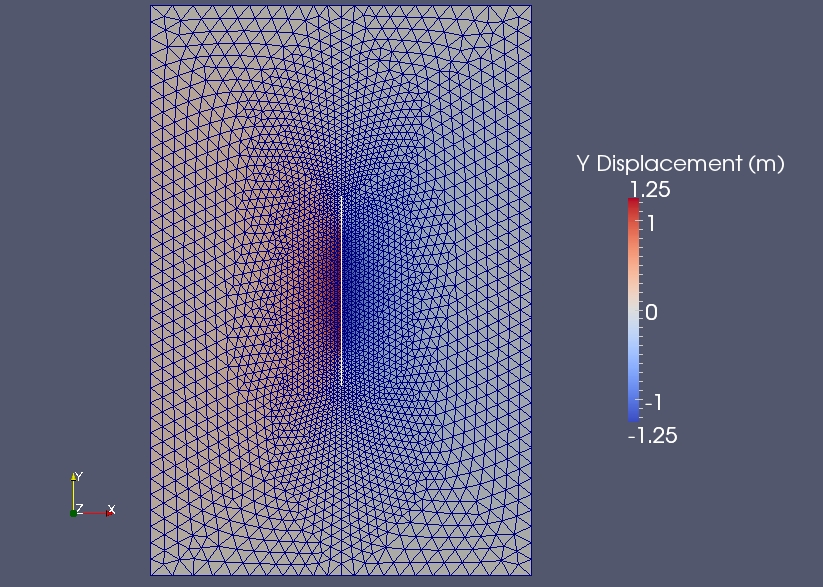
\includegraphics[width=4in]{tutorials/greensfns2d/figs/strikeslip_ydispl2}
\par\end{centering}

\caption{Mesh used for both forward and Green's function computations for the
strike-slip problem. Computed y-displacements for the forward problem
are shown with the color scale.\label{fig:greensfns2d-strikeslip-mesh}}
\end{figure}



\subsection{Additional Common Information}

As in the examples discussed in previous sections of these tutorials,
we place parameters common to the forward model and Green's function
computation in the \texttt{pylithapp.cfg} file so that we do not have
to duplicate them for the two procedures. The settings contained in
\texttt{pylithapp.cfg} for this problem consist of:
\begin{description}
\item [{pylithapp.journal.info}] Settings that control the verbosity of
the output written to stdout for the different components.
\item [{pylithapp.mesh\_generator}] Settings that control mesh importing,
such as the importer type, the filename, and the spatial dimension
of the mesh.
\item [{pylithapp.problem}] Settings that control the problem, such as
the total time, time-step size, and spatial dimension.
\item [{pylithapp.problem.materials}] Settings that control the material
type, specify which material IDs are to be associated with a particular
material type, and give the name of the spatial database containing
the physical properties for the material. The quadrature information
is also given.
\item [{pylithapp.problem.bc}] Settings that control the applied boundary
conditions.
\item [{pylithapp.problem.interfaces}] Settings that control the specification
of faults, including quadrature information.
\item [{pylithapp.problem.formulation.output}] Settings related to output
of the solution over the domain and points (surface observation locations).
\item [{pylithapp.petsc}] PETSc settings to use for the problem, such as
the preconditioner type.
\end{description}
One aspect that has not been covered previously is the specification
of output at discrete points, rather than over a mesh or sub-mesh.
We do this using the \texttt{OutputSolnPoints} output type:
\begin{lyxcode}
{[}pylithapp.problem.formulation{]}

output~=~{[}domain,points{]}

output.points~=~pylith.meshio.OutputSolnPoints



{[}pylithapp.problem.formulation.output.points{]}

coordsys.space\_dim~=~2

coordsys.units~=~km

writer~=~pylith.meshio.DataWriterHDF5

reader.filename~=~output\_points.txt
\end{lyxcode}
We provide the number of spatial dimensions and the units of the point
coordinates, and then the coordinates are given in a simple ASCII
file (\texttt{output\_points.txt}). These same points are used for
both the forward model computation and the generation of the Green's
functions.


\subsection{Step 1: Solution of the Forward Problem}

For both the strike-slip problem and the reverse fault problem, we
first run a static simulation to generate our synthetic data. Parameter
settings that augment those in \texttt{pylithapp.cfg} are contained
in the file \texttt{eqsim.cfg}. These settings are:
\begin{description}
\item [{pylithapp.problem.interfaces}] Give the type of fault interface
condition and provide the slip distribution to use. Linear interpolation
is used for the slip distribution.
\item [{pylithapp.problem.formulation.output}] Gives the output filenames
for domain output, fault output, point output, and material output.
All output uses HDF5 format.
\end{description}
The applied fault slip is given in the file \texttt{eqslip.spatialdb}.
For both the strike-slip and reverse problems, no fault opening is
given, so only the left-lateral component is nonzero. We run the forward
models by typing (in the appropriate directory)
\begin{lyxcode}
pylith~eqsim.cfg
\end{lyxcode}
Once the problem has run, four HDF5 files will be produced. The file
named \texttt{eqsim.h5} (and the associated XDMF file) contains the
solution for the entire domain. This corresponds to the solution shown
in Figure \ref{fig:greensfns2d-strikeslip-mesh}. The \texttt{eqsim-fault.h5}
file contains the applied fault slip and the change in fault tractions,
while the \texttt{eqsim-fault\_info.h5} file contains the final slip,
the fault normal, and the slip time. The final file (\texttt{eqsim-points.h5})
contains the solution computed at the point locations provided in
the \texttt{output\_points.txt} file. These are the results that will
be used as synthetic data for our inversion. One the problem has run,
the results may be viewed with a visualization package such as ParaView.
In Figure \ref{fig:greensfns2d-strikeslip-forward} we show the applied
fault slip (from \texttt{eqsim-fault.h5}) and the resulting x-displacements
(from \texttt{eqsim-points.h5}) for our strike-slip forward problem.

\noindent \begin{center}
\begin{figure}
\begin{centering}
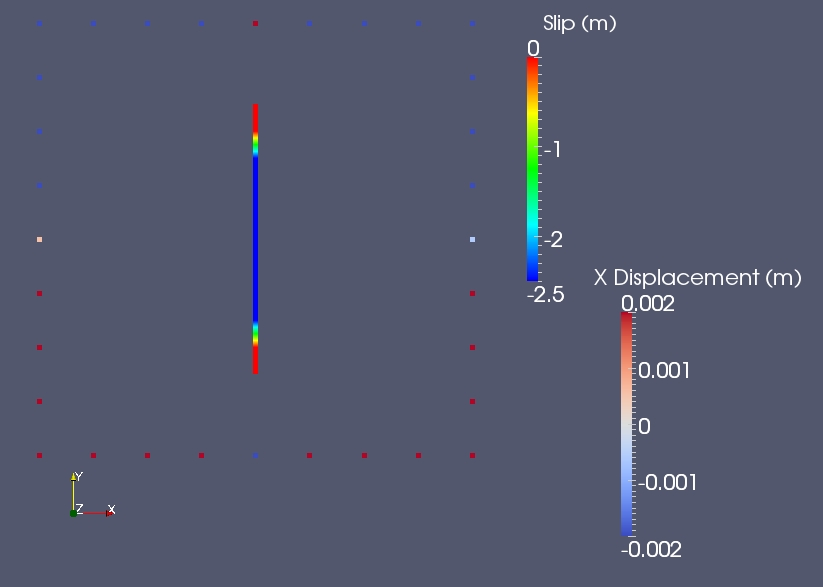
\includegraphics[scale=0.33]{tutorials/greensfns2d/figs/strikeslip_forward_points}
\par\end{centering}

\caption{Applied fault slip for the strike-slip forward problem as well as
computed x-displacements at a set of points.\label{fig:greensfns2d-strikeslip-forward}}
\end{figure}

\par\end{center}


\subsection{Step 2: Generation of Green's Functions}

The next step is to generate Green's functions that may be used in
an inversion. The procedure is similar to that for running the forward
problem; however, it is necessary to change the problem type from
the default \texttt{timedependent} to \texttt{greensfns}. This is
accomplished by simply typing
\begin{lyxcode}
pylith~-{}-problem=pylith.problems.GreensFns
\end{lyxcode}
This changes the problem type and it also causes PyLith to read the
file \texttt{greensfns.cfg} by default, in addition to \texttt{pylithapp.cfg}.
These additional parameter settings provide the information necessary
to generate the Green's functions:
\begin{lyxcode}
{[}greensfns{]}

fault\_id~=~100



\#~Set~the~type~of~fault~interface~condition.

{[}greensfns.interfaces{]}

fault~=~pylith.faults.FaultCohesiveImpulses



\#~Set~the~parameters~for~the~fault~interface~condition.

{[}greensfns.interfaces.fault{]}

\#~Generate~impulses~for~lateral~slip~only,~no~fault~opening.

\#~Fault~DOF~0~corresponds~to~left-lateral~slip.

impulse\_dof~=~{[}0{]}



\#~Set~the~amplitude~of~the~slip~impulses~(amplitude~is~nonzero~on~only

\#~a~subset~of~the~fault)

db\_impulse\_amplitude.label~=~Amplitude~of~slip~impulses

db\_impulse\_amplitude.iohandler.filename~=~impulse\_amplitude.spatialdb

db\_impulse\_amplitude.query\_type~=~nearest
\end{lyxcode}
Note that the top-level identifier is now \texttt{greensfns} rather
than \texttt{pylithapp}. We first set the fault interface condition
type to \texttt{FaultCohesiveImpulses}, and then specify the slip
component to use. The amplitude of the fault slip and the fault vertices
to use are provided in the \texttt{impulse\_amplitude.spatialdb} file.
Fault vertices for which zero slip is specified will not have associated
Green's functions generated. The remainder of the \texttt{greensfns.cfg}
file provides output information, which is exactly analogous to the
settings in \texttt{eqsim.cfg}.

The generation of Green's functions is somewhat similar to the solution
of a time-dependent problem with multiple time steps. In this case,
each `time step' corresponds to the solution computed for a slip impulse
at a particular fault vertex. The output files contain the solution
for each separate impulse (slip on a single fault vertex). The \texttt{greensfns-fault\_info.h5}
file simply contains the slip amplitude and fault normal. In Figure
\ref{fig:greensfns2d-strikeslip-gf6} we show the applied impulse
(from file \texttt{greensfns-fault.h5}) and associated point responses
(from file \texttt{greensfns-points.h5}) for the seventh generated
Green's function in the strike-slip example. In the next section we
will show how to read these Green's functions and use them to perform
a simple linear inversion.

\noindent \begin{center}
\begin{figure}
\begin{centering}
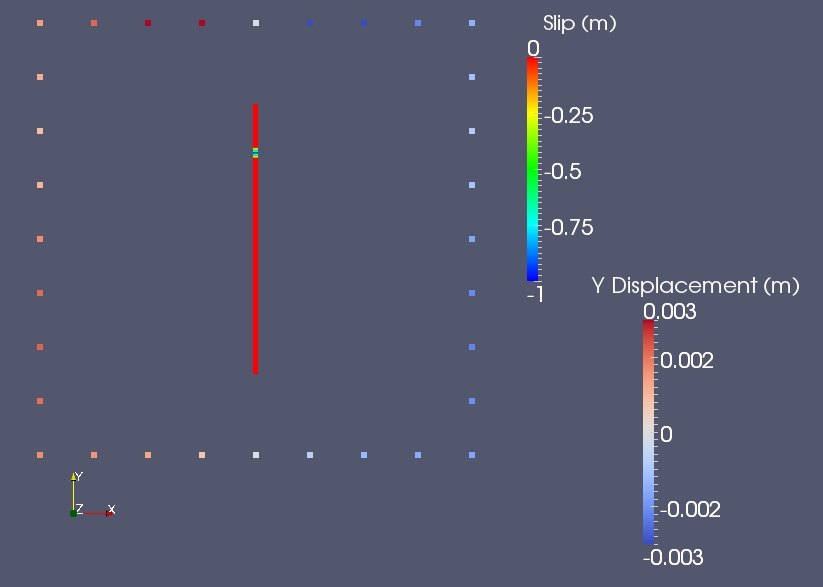
\includegraphics[scale=0.33]{tutorials/greensfns2d/figs/strikeslip_gf6}
\par\end{centering}

\caption{Applied fault slip and computed responses (at points) for the seventh
Green's function generated for the strike-slip fault example.\label{fig:greensfns2d-strikeslip-gf6}}
\end{figure}

\par\end{center}


\subsection{Step 3: Simple Inversion Using PyLith-generated Green's Functions}

In the previous two steps we generated a set of synthetic data as
well as a set of Green's functions. Both are stored in HDF5 files.
To make use of them, we provide a simple Python script that reads
the HDF5 results using the h5py Python package. Once we have read
the necessary information, we will perform a simple least-squares
inversion using the penalty method. We will be solving the equation:
\begin{equation}
G_{a}m=d_{a}\:,
\end{equation}
where $m$ are the model parameters (slip), $G_{a}$ is the augmented
set of Green's functions, and $d_{a}$ is the augmented data vector.
The Green's functions are augmented by the addition of a penalty function:
\begin{equation}
G_{a}=\left[\begin{array}{c}
G\\
\lambda D
\end{array}\right]\:,
\end{equation}
and the data vector is augmented by the addition of the \textit{a
priori} model parameter values:
\begin{equation}
d_{a}=\left[\begin{array}{c}
d\\
m_{ap}
\end{array}\right]\:.
\end{equation}
The matrix $D$ is the penalty function, and $\lambda$ is the penalty
parameter. The solution is obtained using the generalized inverse
(e.g., \cite{Menke:1984}):
\begin{equation}
G^{-g}=\left(G_{a}^{T}G_{a}\right)^{-1}G_{a}^{T}\:,
\end{equation}
and the estimated solution is then:
\begin{equation}
m_{est}=G^{-g}d_{a}\:.
\end{equation}


The code to read the synthetic data and Green's functions and to perform
the inversion is contained in the file \texttt{invert\_slip.py}, which
is contained in the top-level directory. For this simple example,
we have simply used a diagonal matrix as the penalty funtion, and
the \textit{a priori} parameter values are assumed to be zero. The
solution is performed for a range of values of the penalty parameter,
which are contained in the file \texttt{penalty\_params.txt} within
each subdirectory. The inversion is performed by running the script
in the top-level directory from each subdirectory. To run an inversion,
type:
\begin{lyxcode}
../invert\_slip.py~-{}-impulses=output/greensfns-fault.h5~\\
-{}-responses=output/greensfns-points.h5~-{}-data=output/eqsim-points.h5~\\
-{}-penalty=penalty\_params.txt~-{}-output=output/slip\_inverted.txt
\end{lyxcode}
This will produce an ASCII file (\texttt{slip\_inverted.txt}), which
will contain the estimated solution.


\subsection{Step 4: Visualization of Estimated and True Solutions}

Once we have computed the solution, we would then like to visualize
the results. We do this using another Python script that requires
the matplotlib plotting package (this package is not included in the
PyLith binary). We also use the h5py package again to read the applied
slip for the forward problem. The Python code to plot the results
is contained in the \texttt{plot\_invresults.py} file contained within
each subdirectory. To plot the results, type:
\begin{lyxcode}
{\small{}plot\_invresults.py~-{}-solution=output/eqsim-fault.h5~-{}-predicted=output/slip\_inverted.txt}{\small \par}
\end{lyxcode}
The script will produce an interactive matplotlib window that shows
the estimated solution compared to the true solution (Figure \ref{fig:greensfns-invresults}).
As the penalty parameter is increased, the solution is progressively
damped. In a real inversion we would also include the effects of data
uncertainties, and the penalty parameter would represent a factor
controlling the tradeoff between solution simplicity and fitting the
noise in the data.

\noindent \begin{center}
\begin{figure}
\begin{centering}
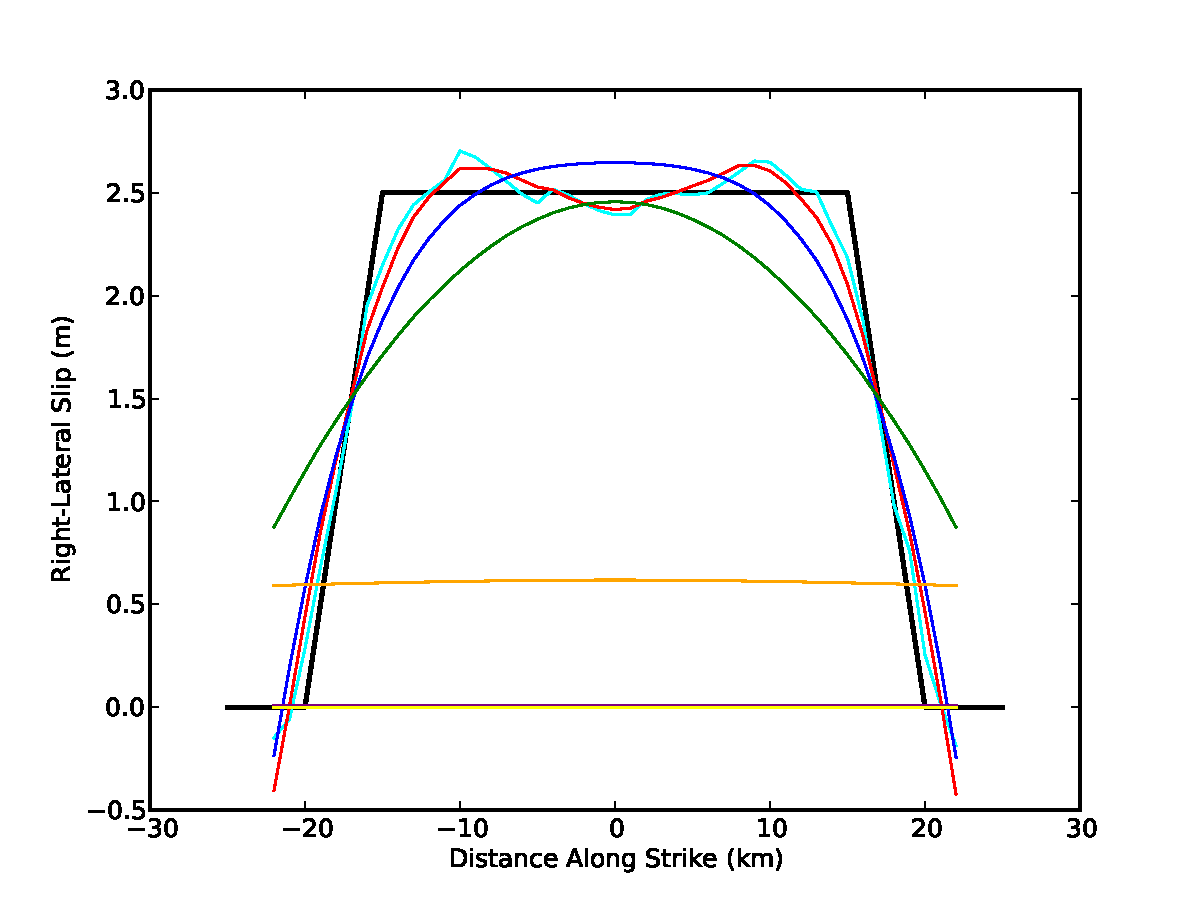
\includegraphics[width=3in]{tutorials/greensfns2d/figs/strikeslip_inversion}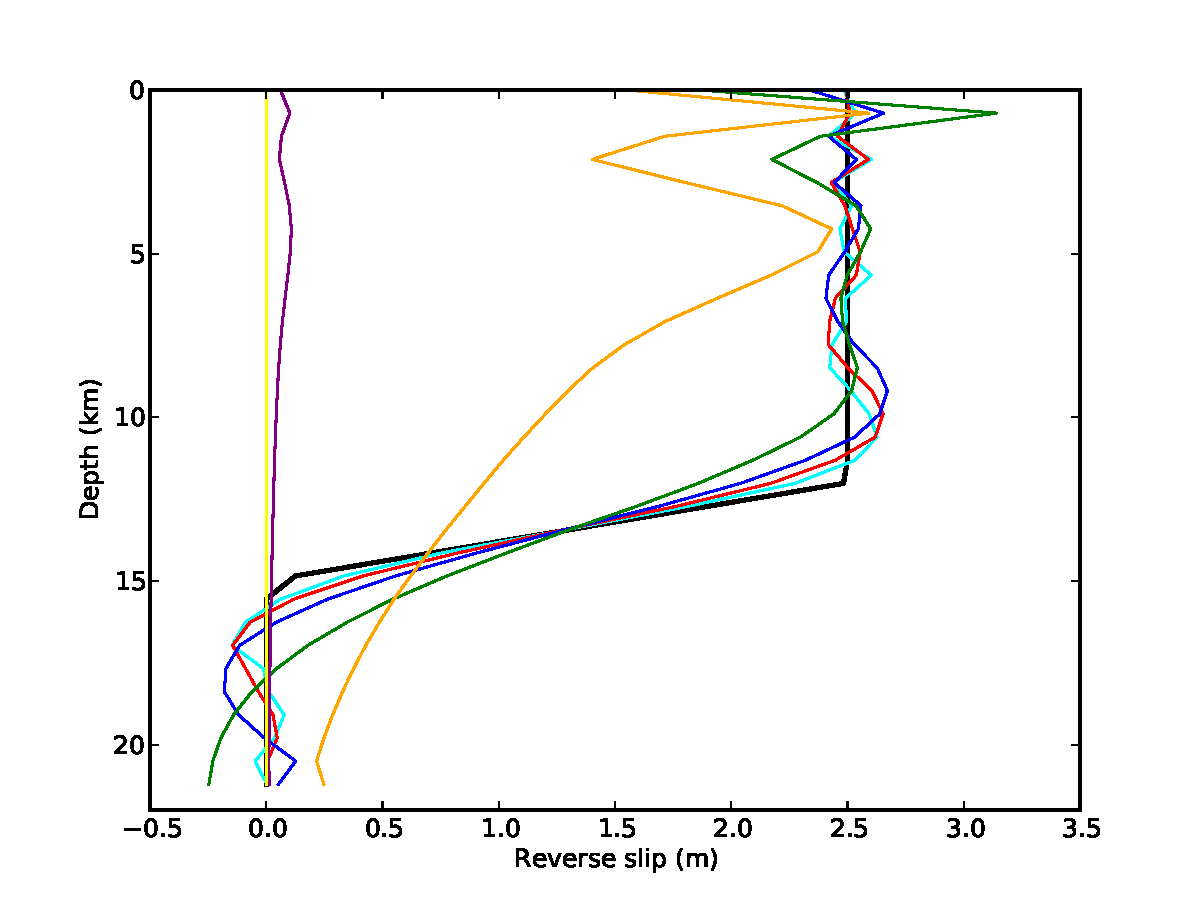
\includegraphics[width=3in]{tutorials/greensfns2d/figs/reverse_inversion}
\par\end{centering}

\caption{Inversion results from running Python plotting script.\label{fig:greensfns-invresults}}
\end{figure}

\par\end{center}
